% \iffalse
\let\negmedspace\undefined
\let\negthickspace\undefined
\documentclass[beamer]{IEEEtran}
\usepackage{cite}
\usepackage{amsmath,amssymb,amsfonts,amsthm}
\usepackage{algorithmic}
\usepackage{graphicx}
\usepackage{textcomp}
\usepackage{xcolor}
\usepackage{txfonts}
\usepackage{listings}
\usepackage{enumitem}
\usepackage{mathtools}
\usepackage{gensymb}
\usepackage{comment}
\usepackage[breaklinks=true]{hyperref}
\usepackage{tkz-euclide} 
\usepackage{listings}
\usepackage{gvv}                                        
\def\inputGnumericTable{}                                 
\usepackage[latin1]{inputenc}                                
\usepackage{color}                                            
\usepackage{array}                                            
\usepackage{longtable}                                       
\usepackage{calc}                                             
\usepackage{multirow}                                         
\usepackage{hhline}                                           
\usepackage{ifthen}                                           
\usepackage{lscape}
\usepackage[export]{adjustbox}

\newtheorem{theorem}{Theorem}[section]
\newtheorem{problem}{Problem}
\newtheorem{proposition}{Proposition}[section]
\newtheorem{lemma}{Lemma}[section]
\newtheorem{corollary}[theorem]{Corollary}
\newtheorem{example}{Example}[section]
\newtheorem{definition}[problem]{Definition}
\newcommand{\BEQA}{\begin{eqnarray}}
\newcommand{\EEQA}{\end{eqnarray}}
\newcommand{\define}{\stackrel{\triangle}{=}}
\theoremstyle{remark}
\newtheorem{rem}{Remark}
\begin{document}
\parindent 0px
\bibliographystyle{IEEEtran}

\title{Assignment\\[1ex]10.5.4-2}
\author{ee23btech11215 - Penmetsa Srikar Varma$^{}$% <-this % stops a space
}
\maketitle
\newpage
\bigskip

\renewcommand{\thefigure}{\theenumi}
\renewcommand{\thetable}{\theenumi}
\section*{Question:}
Q2) The sum of the third and the seventh terms of AP is 6 and their product is 8. Find the sum of first sixteen terms of the AP\\
\section*{Solution:}
{
\centering
Table of Parameters\\
}
\begin{table}[h]
    \centering
    \begin{tabular}{|c|c|}
    \hline
     Input Variables & Input Condition \\
\hline
     x\brak{2}+x\brak{6}& 6 \\
\hline
     x\brak{2}.x\brak{6} & 8 \\
\hline
     $x_i$\brak{n} &  general term of $\text{i}^\text{th}$ AP sequence\\
\hline
     $y_i$\brak{n} &  sum of first n terms of $\text{i}^\text{th}$ AP sequence\\
\hline
     $x_i$\brak{0} & first term of $\text{i}^\text{th}$ AP sequence\\
\hline
     $d_i$ & common difference of $\text{i}^\text{th}$ AP sequence\\
\hline
     $x_i\brak{n}\system{Z}X_i\brak{z}$ & $z$-transform of $x_i\brak{n}$ \\
\hline
     $y_i\brak{n}\system{Z}Y_i\brak{z}$ & $z$-transform of $y_i\brak{n}$ \\
\hline
    \end{tabular}

    \label{tab:my_label}
\end{table}

Then general term x\brak{n} of arithmetic progression is given by:
\begin{align}
\label{q1}
x\brak{n}&=x\brak{0}+n.d
\end{align}
 
Then from table of parameters,
\begin{align}
\label{q6}
    x\brak{2}&=6-x\brak{6}
\end{align}
From \brak{\ref{q6}}
\begin{align}
x\brak{2}.x\brak{6}=8
\end{align}
\begin{align}
\label{q7}
    x\brak{6}&=2\ \text{or}\ 4
\end{align}
Then from $\brak{\ref{q6}}$ and $\brak{\ref{q7}}$
\begin{align}
\label{q8}
    x\brak{2}&=4\ \text{or}\ 2
\end{align}
for x$\brak{2}$ = 2 and x$\brak{6}$ = 4
\begin{align}
x\brak{0}&=1,\ d=\frac{1}{2}
\end{align}
for x$\brak{2}$ = 4 and x$\brak{6}$ = 2
\begin{align}
x\brak{0}&=5,\ d=-\frac{1}{2}
\end{align}
We know that the sum of first n terms of arithmetic progression is given by:
\begin{align}
\label{q9}
S\brak{n}&= \frac{n}{2}\brak{2x\brak{0}+\brak{n-1}d}u\brak{n}
\end{align}
Then from \brak{\ref{q9}}
\begin{align}
\label{q10}
S\brak{16}&= \frac{16}{2}\brak{2.x\brak{0}+15d}
\end{align}
Hence from \brak{\ref{q10}},
for $x\brak{0}$=1,d=$\frac{1}{2}$
\begin{align}
\label{11}
S_1\brak{16}&=76
\end{align}
or from \brak{\ref{q10}},
for $x\brak{0}$=5,d=-$\frac{1}{2}$
\begin{align}
\label{12}
S_2\brak{16}&=20
\end{align}
The general term of AP x\brak{n} and sum of first n terms of AP S\brak{n} are given by:
\begin{align}
x_1\brak{n}&=\brak{\frac{n+2}{2}}u\brak{n}\ \text{and}\ S_1\brak{n}=\brak{\frac{n\brak{n+3}}{4}}u\brak{n}
\end{align}
\begin{align}
x_2\brak{n}&=\brak{\frac{10-n}{2}}u\brak{n}\ \text{and}\ S_2\brak{n}=\brak{\frac{n\brak{21-n}}{4}}u\brak{n}
\end{align}

\begin{figure}[h]
    \centering
    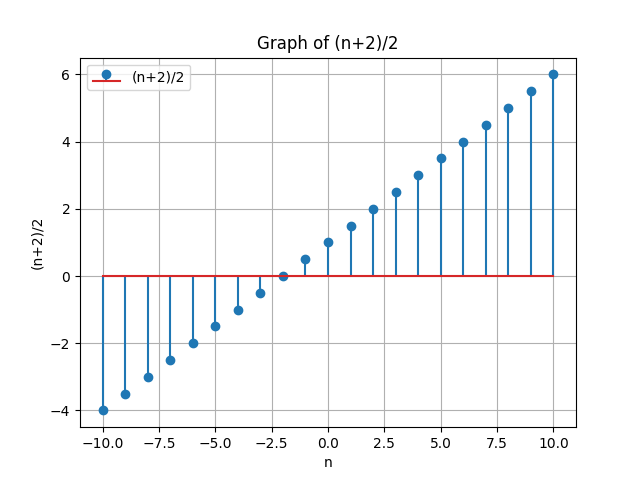
\includegraphics[scale=0.60]{py_3.png}
    \label{fig:x1n}
    \caption*{Graph of $x_1\brak{n}$}
\end{figure}

\begin{figure}[h]
    \centering
    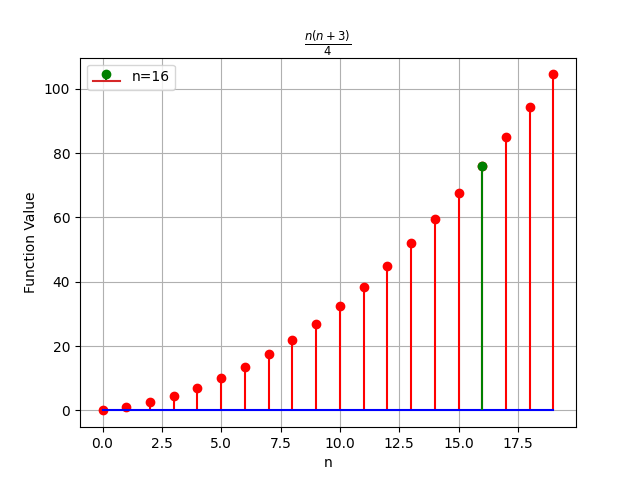
\includegraphics[scale=0.60]{py_4.png}
    \label{fig:s1n}
    \caption*{Graph of $S_1\brak{n}$}
\end{figure}

\begin{figure}[h]
    \centering
    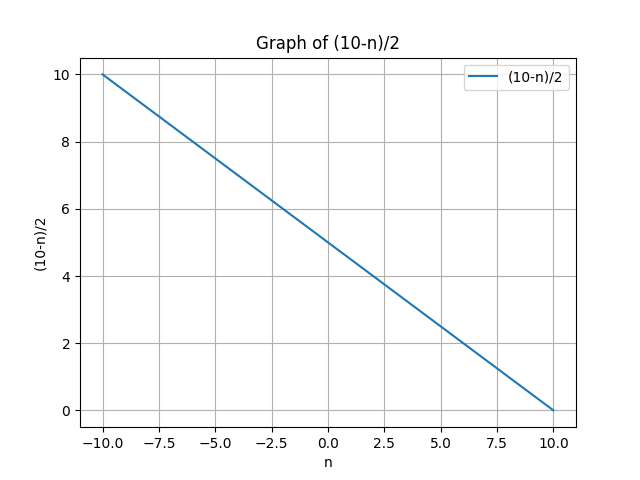
\includegraphics[scale=0.60]{py_5.png}
    \label{fig:x2n}
    \caption*{Graph of $x_2\brak{n}$}
\end{figure}

\begin{figure}[h]
    \centering
    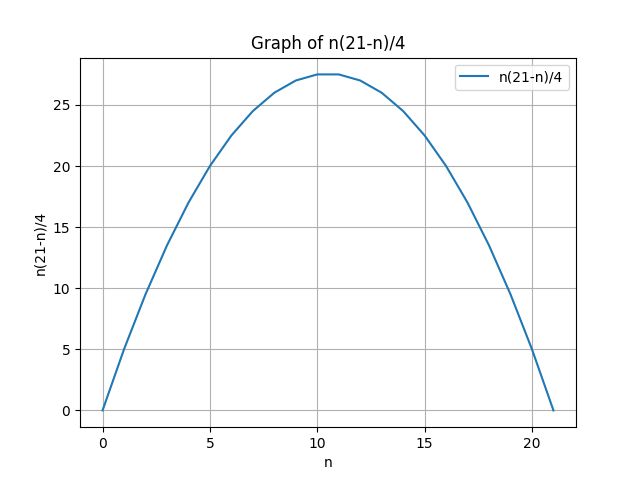
\includegraphics[scale=0.60]{py_6.png}
    \label{s2n}
    \caption*{Graph of $S_2\brak{n}$}
\end{figure}
We know that Z-Transform of x\brak{n} is given by:
\begin{align}
\label{q11}
    X\brak{z}&=\sum_{k=-\infty}^{\infty} x\brak{k}z^{-k}
\end{align}

\begin{align}
\label{q12}
    X_1\brak{z}&=\sum_{k=0}^{\infty} x_1\brak{k}z^{-k}
\end{align}
\begin{align}X_1\brak{z}&=\sum_{k=0}^{\infty} \brak{\frac{k+2}{2}}u\brak{k}z^{-k}\end{align}
\begin{align}
    \label{q13}
    X_1\brak{z}&=\frac{1}{2}\brak{\sum_{k=0}^{\infty}k\ u\brak{k}z^{-k}}+\sum_{k=0}^{\infty}u\brak{k}z^{-k}
\end{align}
\begin{align}
    \label{q13}
    X_1\brak{z}&=\frac{1}{2}\brak{\frac{z^{-1}}{\brak{1-z^{-1}}^2}}+\frac{1}{1-z^{-1}}
\end{align}
So,
\begin{align} X_1\brak{Z}&=\frac{2-z^{-1}}{2.\brak{1-z^{-1}}^2},\text{ROC}\implies\{|z^{-1}|<1\}\end{align}

From \brak{\ref{q12}},
\begin{align}
    X_2\brak{z}&=\sum_{k=0}^{\infty} x_2\brak{k}z^{-k}
\end{align}
\begin{align}X_2\brak{Z}&=\sum_{k=0}^{\infty} \brak{\frac{10-k}{2}}u\brak{k}z^{-k}\end{align}
\begin{align}X_2\brak{Z}&=5\brak{\sum_{k=0}^{\infty}u\brak{k}z^{-k}}-\frac{1}{2}\brak{\sum_{k=0}^{\infty}k\ u\brak{k}z^{-k}}\end{align}
So,
\begin{align}X_2\brak{Z}&=\frac{10-11z^{-1}}{2.\brak{1-z^{-1}}^2},\text{ROC}\implies\{|z^{-1}|<1\}\end{align}
\begin{figure}[h]
    \centering
    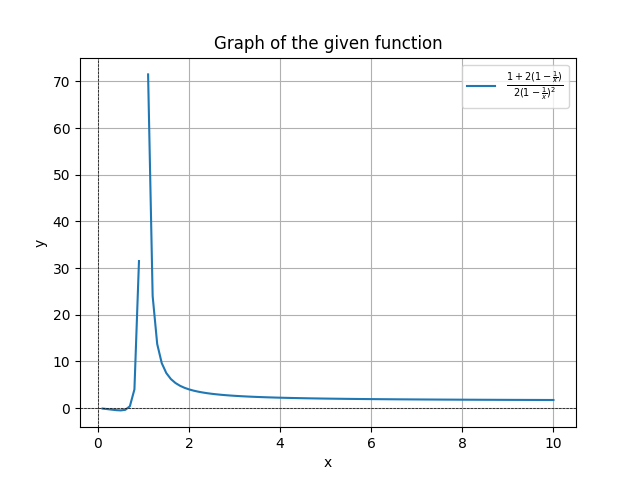
\includegraphics[scale=0.52]{py_31.png}
    \label{fig:x1z}
    \caption*{Graph of $X_1\brak{Z}$}
\end{figure}
\begin{figure}[h]
    \centering
    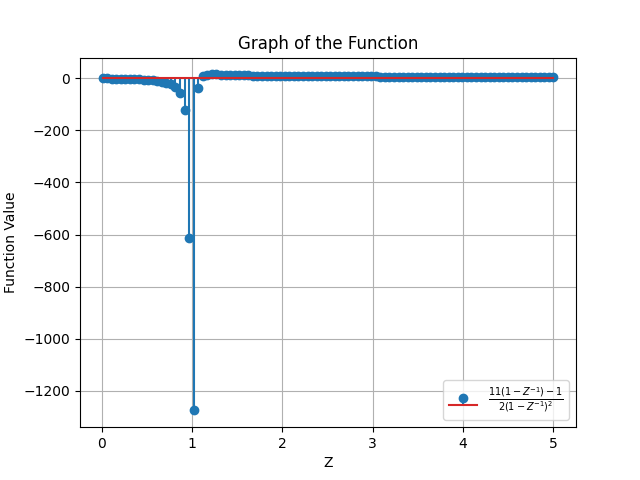
\includegraphics[scale=0.52]{py_32.png}
    \label{x2z}
    \caption*{Graph of $X_2\brak{Z}$}
\end{figure}

Let, $\mathcal{Z}$ transform of s(n) be S(Z):\\
from \brak{\ref{q11}}:
$$S\brak{Z}=\sum_{k=-\infty}^{\infty}s(k)\ z^{-k}$$
from \brak{\ref{q9}}
\begin{align}
S\brak{Z}&=\sum_{k=-\infty}^{\infty}\left(\brak{x\brak{0}-\frac{d}{2}}k+\frac{d}{2}\ k^2\right)u\brak{k}z^{-k}
\end{align}

\begin{align}
\label{q17}
    S\brak{Z}&=\brak{x\brak{0}-\frac{d}{2}}\left(\sum_{k=0}^{\infty}kz^{-k}\right)+\frac{d}{2}\left(\sum_{k=0}^{\infty}k^2z^{-k}\right)
\end{align}

\begin{align}
\label{w1}
s\brak{Z}&=x\brak{0}\brak{\frac{z}{\brak{z-1}^2}}+d\brak{\frac{z}{\brak{z-1}^3}}
\end{align}

for x\brak{0}=1 and $d=\frac{1}{2}$

\begin{align}
S_1\brak{Z}&=\frac{z\brak{z-\frac{1}{2}}}{\brak{z-1}^3},\text{ROC}\implies\{|z|>1\}
\end{align}

\begin{figure}[h]
    \centering
    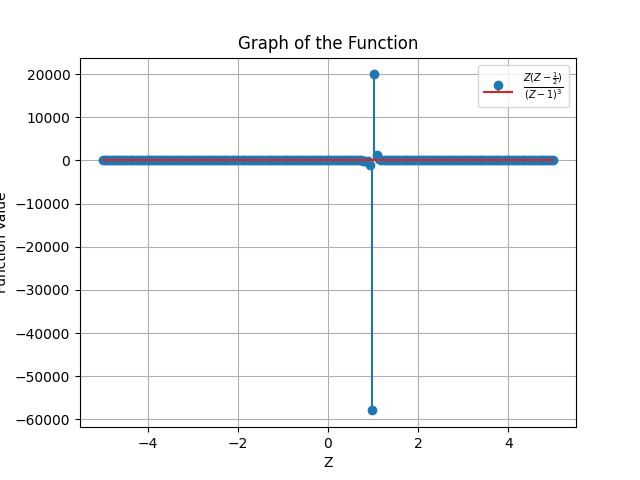
\includegraphics[scale=0.52]{py_33.png}
    \label{fig:s1z}
    \caption*{Graph of $S_1\brak{Z}$}
\end{figure}

for x\brak{0}=5 and $d=-\frac{1}{2}$

\begin{align}S_2\brak{Z}&=\frac{z\brak{5z-\frac{11}{2}}}{\brak{z-1}^3},\text{ROC}\implies\{|z|>1\}\end{align}

\begin{figure}[h]
    \centering
    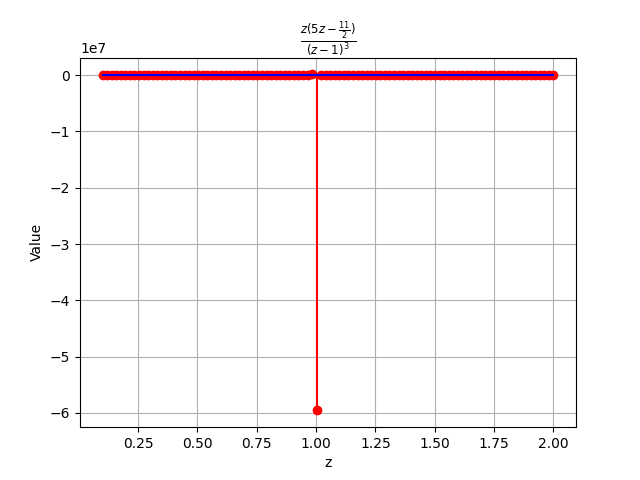
\includegraphics[scale=0.52]{py_34.png}
    \label{fig:s2z}
    \caption*{Graph of $S_2\brak{Z}$}
\end{figure}

We know that Inverse $\mathcal{Z}$ - transform of $S\brak{z}$ say $s\brak{n}$, by counter integral method is given by:

\begin{align}
s\brak{n}&=\oint_C S(z)\ z^{n-1}\, dz
\end{align}

from \brak{\ref{w1}},

\begin{align}
    s\brak{n}&=x\brak{0}\oint_C \brak{\frac{z}{\brak{z-1}^2}dz} + d\brak{\oint_C  \frac{z}{\brak{z-1}^3} \, dz}
\end{align}

We can observe that pole is repeated 2,3 times\\so, m=2 and 3 respectively:
\begin{align}
    s\brak{n}&=x\brak{0}\left|\frac{1}{1!}\frac{d}{dz}\brak{z^n}\right|_{z=1} + d\left|\frac{1}{2!}\frac{d^2}{dz^2}\brak{z^n}\right|_{z=1}
\end{align}

\begin{align}
    s\brak{n}&=\brak{n\ x\brak{0} + n\brak{n-1}\frac{d}{2}}u\brak{n}
\end{align}
\begin{align}
\label{39}
    s_1\brak{n}&=\frac{n\brak{n+3}}{4}u\brak{n},s_1\brak{16}=76
\end{align}
and,
\begin{align}
\label{40}
    s_2\brak{n}&=\frac{n\brak{21-n}}{4}u\brak{n},s_2\brak{16}=20
\end{align}

we can observe that \brak{\ref{11}} and \brak{\ref{39}},\brak{\ref{12}} and \brak{\ref{40}} are the same results
\end{document}
